% id: 0289
% book: RPM 중3-2 수학 · 03 원과 직선
% section: 유형 07 원의 접선의 길이 (1)
% figure: crop:fig-0289.png
% answer: ②
% answer_source: 답지
% variant_level: 0 (원본 전사)
% 이 파일은 build.mjs 가 items.json 에서 만든다. 고칠 때는 items.json 을 고친다.
\smash{\raisebox{1.5mm}{\dmkichul{대표문제}}}
\noindent\begin{minipage}[t]{0.58\linewidth}\vspace{0pt}\raggedright 오른쪽 그림과 같이 반지름의 길이가 $3\mkern3mu \mathrm{cm}$인 원~$\pt{O}$에서 점~$\pt{A}$는 원~$\pt{O}$의 접점이고 $\seg{PQ}=4\mkern3mu \mathrm{cm}$일 때, $\seg{AP}$의 길이는?\end{minipage}\hfill\begin{minipage}[t]{0.4\linewidth}\vspace{0pt}\centering \setlength{\dmfigw}{88.5pt}\ifdim\dmfigw>\linewidth\setlength{\dmfigw}{\linewidth}\fi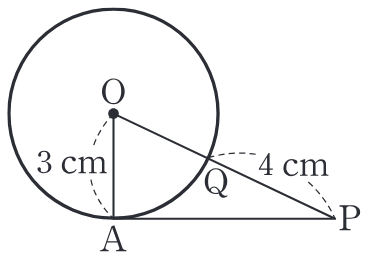
\includegraphics[width=\dmfigw]{figures/fig-0289.png}\end{minipage}\par
\begin{choices32}{\rule[-3ex]{0pt}{8ex}$6\mkern3mu \mathrm{cm}$}{\rule[-3ex]{0pt}{8ex}$2\sqrt{10}\mkern3mu \mathrm{cm}$}{\rule[-3ex]{0pt}{8ex}$4\sqrt{3}\mkern3mu \mathrm{cm}$}{\rule[-3ex]{0pt}{8ex}$7\mkern3mu \mathrm{cm}$}{\rule[-3ex]{0pt}{8ex}$5\sqrt{2}\mkern3mu \mathrm{cm}$}\end{choices32}
